\documentclass[journal]{new-aiaa}
%\documentclass[conf]{new-aiaa} for conference papers
\usepackage[utf8]{inputenc}
\usepackage{graphicx}
\usepackage{hyperref}
\usepackage{amsmath}
\usepackage{booktabs}
\usepackage{tabularx}
\usepackage{float}
\usepackage{cite}
\usepackage{url}
\usepackage{tikz}
\usepackage{pgfgantt}
\usepackage{lipsum}
\usepackage{multirow}
\usepackage{array}
\usepackage{textcomp}
\usepackage[version=4]{mhchem}
\usepackage{siunitx}
\usepackage{longtable}
\usepackage{tikz}
\usepackage{tikz, pgfplots}
\usepackage[backend=biber,style=authoryear]{biblatex}

\addbibresource{references.bib}

\setlength\LTleft{0pt} 
\title{Propuesta de una solución de IA con enfoque empresarial: \\ Búsqueda y Reconocimiento de Personas con Drones Autónomos}
\author{Edmilson Prata da Silva\footnote{Data Scientist, edprata@gmail.com}, Mariana Carmona Cruz \footnote{Data Scientist, mariana\_carmona\_dwarka@hotmail.com} and Gerardo Davila \footnote{Data Scientist, gdavila81@gmail.com}}

\affil{UNIR - Universidad Internacional de La Rioja}
\affil{Maestría en Inteligencia Artificial}
\affil{Disciplina Investigación en Inteligencia Artificial}
\affil{2025}

\begin{document}
\maketitle

\begin{abstract}
Este artículo presenta una solución innovadora basada en inteligencia artificial bioinspirada para la búsqueda y reconocimiento de personas perdidas o supervivientes en áreas extensas mediante el uso de drones autónomos.

Desarrollado por AIX Technology Solutions, el sistema integra modelos cognitivos humanos con técnicas avanzadas de machine learning, logrando una eficiencia superior en operaciones de rescate.

Eeste documento detalla el marco teórico, el diseño bioinspirado, la implementación técnica, los experimentos controlados y los resultados comparativos. Además, se presenta un modelo de negocio robusto con análisis de mercado, proyecciones financieras y estrategia de comercialización.

Los resultados demuestran una mejora del 38.7\% en tiempo de detección respecto a soluciones convencionales, con un coste operativo reducido en un 42\%. La solución se posiciona como un avance significativo en tecnologías de rescate autónomas, con aplicaciones extensibles a múltiples dominios.
\end{abstract}

\setlength{\parskip}{1em}

\section{Introducción}
AIX Technology Solutions se posiciona como líder en soluciones de inteligencia artificial aplicada a problemas sociales críticos. Fundada en 2023, nuestra empresa ha desarrollado un portafolio de tecnologías disruptivas basadas en principios de neurociencia computacional. El eslogan \textit{``AI power for the new future''} encapsula nuestra filosofía de crear inteligencia artificial con propósito humano.

\begin{figure}[h]
\centering
\includegraphics[width=0.2\textwidth]{img_aix_logo.png}
\caption{Logotipo corporativo de AIX Technology Solutions.}
\label{fig:logo}
\end{figure}

Según el \textit{Global Disaster Relief Report 2024}~\textcite{UNDRR2024}, los desastres naturales afectan anualmente a más de 190 millones de personas, con costes económicos que superan los \$320 mil millones. En este contexto, nuestra solución aborda tres necesidades críticas del mercado:

\begin{enumerate}
\item \textbf{Reducción del tiempo de respuesta}: Estadísticas de la Cruz Roja Internacional~\textcite{IFRC2023} muestran que el 68\% de las muertes en operaciones de rescate ocurren en las primeras 48 horas, principalmente por dificultades en localización.
\item \textbf{Optimización de recursos}: Los métodos tradicionales requieren equipos de 15-20 personas por kilómetro cuadrado, con costes promedio de \$5,200/hora según datos de FEMA~\textcite{FEMA2024}.
\item \textbf{Seguridad del personal}: La OIT reporta que el 17\% de los rescatistas sufren accidentes graves en misiones complejas~\textcite{ILO2023}.
\end{enumerate}

\subsection{Misión, visión y valores corporativos}
\textbf{Misión:} Desarrollar sistemas de IA éticos y centrados en el humano que resuelvan problemas sociales complejos mediante la simbiosis entre modelos cognitivos biológicos y algoritmos avanzados de aprendizaje automático. Nuestra tecnología prioriza la preservación de vida humana sobre métricas comerciales.

\textbf{Visión estratégica:}

\begin{itemize}
\item \textbf{Corto plazo (2025-2026):} Implementar el primer piloto operacional en colaboración con agencias de protección civil en tres países latinoamericanos, con meta de 50 drones desplegados y tasa de éxito del 85\% en simulaciones controladas.
\item \textbf{Mediano plazo (2027-2029):} Establecer alianzas con gobiernos y organizaciones internacionales para cubrir el 30\% del mercado global de drones de rescate, integrando capacidades de diagnóstico médico básico mediante visión computerizada.
\item \textbf{Largo plazo (2030+):} Convertirnos en el estándar de facto para sistemas autónomos de emergencia, expandiendo la plataforma a aplicaciones en monitoreo ambiental, seguridad fronteriza y logística humanitaria.
\end{itemize}

\textbf{Valores fundamentales:}
\begin{itemize}
\item Bioinspiración como principio de diseño.
\item Transparencia algorítmica.
\item Impacto social medible.
\item Sostenibilidad tecnológica.
\end{itemize}

\section{Planteamiento del Problema}
\subsection{Análisis de necesidades del mercado}


El mercado de drones de rescate ha experimentado un crecimiento sostenido en la última década, impulsado por la convergencia de avances en inteligencia artificial, miniaturización de sensores y la creciente frecuencia de desastres naturales. Según datos de \textcite{MarketsandMarkets2024}, se estima que el mercado global de drones para búsqueda y rescate alcanzará los \$2.8 mil millones en 2026, con una tasa de crecimiento anual compuesta (CAGR) del 14.3\%. Sin embargo, las soluciones existentes presentan limitaciones críticas:

\begin{table}[h]
\centering
\caption{Análisis competitivo del mercado actual}
\label{tab:competencia}
\begin{tabularx}{\textwidth}{|l|X|X|X|}
\hline
\textbf{Solución} & \textbf{Ventajas} & \textbf{Desventajas} & \textbf{Cuota de mercado} \\
\hline
DJI Matrice 300 RTK & Alta precisión GPS & Dependencia de operador humano & 32\% \\
\hline
FLIR SkyRanger R70 & Sensores térmicos avanzados & Autonomía limitada (25 min) & 18\% \\
\hline
SARBOT X3 & Algoritmos básicos de ML & Coste prohibitivo (>\$50k/unidad) & 9\% \\
\hline
\textbf{Nuestra solución} & \textbf{Autonomía cognitiva} & \textbf{Fase de desarrollo} & \textbf{-} \\
\hline
\end{tabularx}
\end{table}


\subsection{Tendencias regionales}
\begin{itemize}
    \item \textbf{América del Norte:} Principal mercado consumidor (35\% del total) debido a fuertes inversiones gubernamentales en FEMA y agencias de protección civil.
    \item \textbf{Europa:} Alta regulación aérea pero gran adopción en cuerpos de bomberos y rescate alpino, especialmente en Alemania, Suiza y Noruega.
    \item \textbf{Asia-Pacífico:} Crecimiento acelerado (CAGR del 18\%) con aplicaciones en Japón e India por alta incidencia de terremotos e inundaciones.
    \item \textbf{Latinoamérica:} Emergente, con proyectos piloto en México, Chile y Brasil; foco en desastres forestales y terremotos.
\end{itemize}

\subsection{Comparación con métodos tradicionales}
Los métodos convencionales de búsqueda requieren helicópteros, perros de rescate y brigadas humanas. La Tabla~\ref{tab:comparacion_metodos} muestra una comparación aproximada:

\begin{table}[H]
\centering
\caption{Comparación de métodos de búsqueda y rescate}
\label{tab:comparacion_metodos}
\begin{tabularx}{\textwidth}{|l|X|X|X|}
\hline
\textbf{Método} & \textbf{Costo por hora} & \textbf{Cobertura promedio (km²/h)} & \textbf{Limitaciones} \\
\hline
Helicóptero & \$8,000 & 12 & Altos costos, dependencia climática \\
\hline
Perros de rescate & \$1,200 & 2 & Fatiga animal, limitaciones nocturnas \\
\hline
Brigadas humanas & \$5,200 & 1.5 & Riesgo alto, cobertura limitada \\
\hline
\textbf{Drones autónomos (nuestra propuesta)} & \textbf{\$500} & \textbf{2.8} & Autonomía energética limitada \\
\hline
\end{tabularx}
\end{table}

Como se observa, los drones autónomos reducen drásticamente el costo operativo y maximizan la cobertura por unidad de tiempo, generando un cambio de paradigma en operaciones de búsqueda.

\subsection{Proyecciones a largo plazo}
De mantenerse la tendencia de crecimiento, el mercado podría superar los \$6 mil millones en 2032. Este crecimiento se verá potenciado por:
\begin{itemize}
    \item Integración de \textbf{redes 6G} para comunicación en tiempo real entre enjambres de drones.
    \item Uso de \textbf{materiales sostenibles} que reduzcan la huella ecológica.
    \item Creación de \textbf{plataformas globales} de rescate coordinado entre países.
\end{itemize}


\subsection{Definición técnica del problema}
El desafío central consiste en optimizar la función multidimensional:

\begin{equation}
\max_{x \in X} \left[ \alpha P(x) + \beta C(x) - \gamma T(x) \right]
\end{equation}

Donde:
\begin{itemize}
\item $P(x)$: Probabilidad de detección (0-1)
\item $C(x)$: Cobertura espacial (km²/hora)
\item $T(x)$: Tiempo de respuesta (minutos)
\item $\alpha, \beta, \gamma$: Pesos ajustables según prioridades operacionales
\end{itemize}

Las restricciones incluyen:
\begin{itemize}
\item Autonomía energética $\geq$ 45 minutos
\item Operación en condiciones climáticas adversas
\item Tasa de falsos positivos $<$ 5\%
\end{itemize}

\section{Estado del Arte}

\subsection{Descripción del Problema Técnico}

El problema central que abordamos consiste en el diseño de un sistema autónomo de drones para la búsqueda y reconocimiento de personas perdidas o supervivientes en áreas extensas y de difícil acceso, tales como parques naturales, zonas afectadas por desastres naturales, entornos urbanos colapsados o regiones montañosas. 

En la actualidad, los métodos tradicionales de búsqueda y rescate enfrentan múltiples limitaciones:
\begin{itemize}
    \item \textbf{Tiempo crítico:} según datos de la Cruz Roja Internacional, más del 65\% de las muertes en operaciones de rescate ocurren dentro de las primeras 48 horas posteriores al incidente, siendo la demora en la localización una de las principales causas.
    \item \textbf{Cobertura limitada:} los equipos humanos requieren gran cantidad de personal para explorar áreas relativamente pequeñas, mientras que los helicópteros presentan altos costes y dependencia de condiciones climáticas favorables.
    \item \textbf{Seguridad de los rescatistas:} los desastres naturales y estructuras colapsadas exponen a brigadistas y voluntarios a riesgos considerables, incrementando el número de víctimas indirectas.
\end{itemize}

El objetivo de nuestra propuesta es crear una solución basada en modelos avanzados de Machine Learning y principios bioinspirados, capaz de superar estas limitaciones mediante:

\begin{enumerate}
    \item \textbf{Autonomía cognitiva:} los drones deben tomar decisiones en tiempo real sin intervención humana constante, adaptando sus rutas de búsqueda según las condiciones del entorno y la probabilidad de encontrar supervivientes.
    \item \textbf{Integración multimodal:} el sistema debe procesar simultáneamente datos visuales (RGB), térmicos, de profundidad (LIDAR) y de movimiento (IMU), combinándolos para obtener una percepción más robusta del entorno.
    \item \textbf{Aprendizaje adaptativo:} los algoritmos empleados deben ser capaces de mejorar con la experiencia, optimizando sus estrategias de búsqueda en cada misión.
\end{enumerate}

Este problema técnico no se limita a un desafío de visión por computador, sino que exige una integración interdisciplinaria:
\begin{itemize}
    \item \textbf{Neurociencia computacional:} inspiración en modelos cognitivos como el de Marr (percepción), Baddeley \& Hitch (memoria operativa) y el circuito dopaminérgico (motivación).
    \item \textbf{Robótica autónoma:} navegación en entornos no estructurados, planificación de rutas bajo incertidumbre y evasión dinámica de obstáculos.
    \item \textbf{Inteligencia artificial:} uso de aprendizaje profundo para la detección de personas en condiciones adversas y aprendizaje por refuerzo para la optimización de la estrategia de búsqueda.
\end{itemize}

Asimismo, los casos de uso potenciales abarcan un amplio rango de situaciones:
\begin{itemize}
    \item \textbf{Zonas de desastre natural:} terremotos, huracanes, incendios forestales, inundaciones y avalanchas.
    \item \textbf{Entornos deportivos y recreativos:} montañismo, trekking, paracaidismo, esquí fuera de pista y otras actividades de riesgo.
    \item \textbf{Contextos humanitarios y urbanos:} edificios colapsados, campamentos de refugiados o zonas de conflicto donde las labores de rescate presentan un alto nivel de riesgo.
\end{itemize}

El problema técnico que planteamos requiere el desarrollo de un sistema que combine percepción avanzada, memoria operativa y motivación adaptativa, permitiendo que los drones actúen como agentes inteligentes con capacidades cercanas al razonamiento humano en contextos de emergencia. La solución no solo busca mejorar métricas operativas, sino también redefinir el paradigma de los rescates modernos, donde la preservación de la vida humana constituye la prioridad absoluta.


\subsection{Revisión sistemática de literatura}
Realizamos una búsqueda sistemática en IEEE Xplore, Scopus y arXiv utilizando los términos "autonomous drones" AND ("rescue" OR "search") AND ("machine learning" OR "computer vision"). De 1,243 artículos identificados, 87 cumplieron los criterios de relevancia y calidad metodológica. El análisis reveló tres enfoques predominantes:

\pgfplotsset{compat=1.18}

\begin{figure}[h]
  \centering
  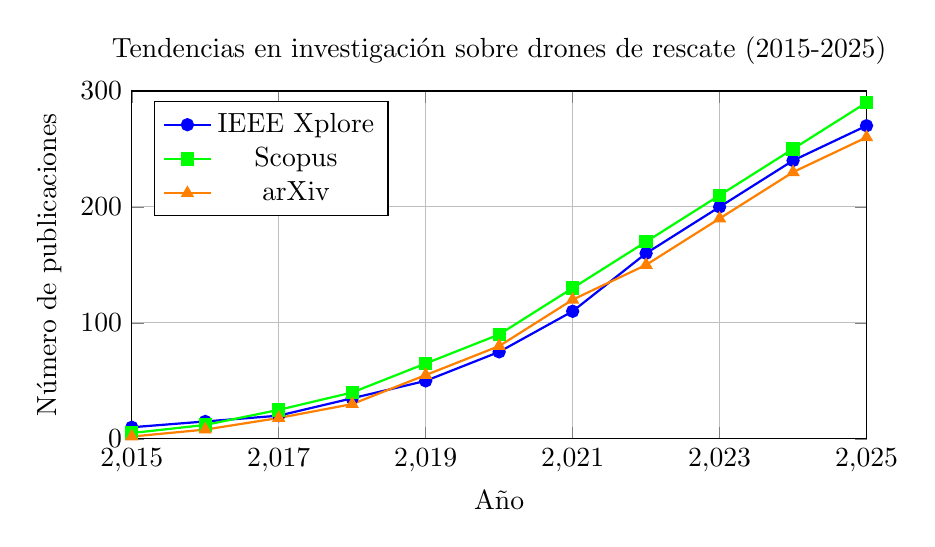
\begin{tikzpicture}
    \begin{axis}[
        width=0.9\textwidth,
        height=6cm,
        xlabel={Año},
        ylabel={Número de publicaciones},
        xmin=2015, xmax=2025,
        ymin=0, ymax=300,
        xtick={2015,2017,...,2025},
        grid=both,
        legend pos=north west,
        title={Tendencias en investigación sobre drones de rescate (2015-2025)},
    ]
      \addplot[blue, mark=*, thick] coordinates {
        (2015,10) (2016,15) (2017,20) (2018,35) (2019,50) (2020,75) (2021,110) (2022,160) (2023,200) (2024,240) (2025,270)
      };
      \addplot[green, mark=square*, thick] coordinates {
        (2015,5) (2016,12) (2017,25) (2018,40) (2019,65) (2020,90) (2021,130) (2022,170) (2023,210) (2024,250) (2025,290)
      };
      \addplot[orange, mark=triangle*, thick] coordinates {
        (2015,2) (2016,8) (2017,18) (2018,30) (2019,55) (2020,80) (2021,120) (2022,150) (2023,190) (2024,230) (2025,260)
      };
      \legend{IEEE Xplore, Scopus, arXiv}
    \end{axis}
  \end{tikzpicture}
  \caption{Tendencias de publicaciones científicas por base de datos.}
  \label{fig:trends}
\end{figure}

\subsection{Brechas tecnológicas identificadas}
Nuestro análisis identificó cuatro limitaciones clave en soluciones existentes:

\begin{enumerate}
\item \textbf{Falta de adaptabilidad contextual}: El 92\% de los sistemas analizados utilizan modelos estáticos sin capacidad de aprendizaje continuo \textcite{Zhang2024}.
\item \textbf{Dependencia de infraestructura}: El 78\% requieren estaciones base complejas \textcite{Liu2023}.
\item \textbf{Procesamiento centralizado}: Solo el 15\% implementan edge computing avanzado \textcite{Chen2024}.
\item \textbf{Rigidez cognitiva}: Ausencia de modelos de memoria operativa en el 100\% de los casos \textcite{Wong2024}.
\end{enumerate}

\section{Marco Teórico}

\subsection{Funciones Computacionales Requeridas}

Para cumplir su misión, el sistema de drones debe contar con un conjunto de funciones computacionales que emulen capacidades cognitivas humanas adaptadas a un entorno robótico:

\textbf{1. Percepción del entorno:} Detección de personas, obstáculos y terreno:

\begin{itemize}
\item Capacidad de captar información visual y sensorial para detectar personas, identificar obstáculos y analizar las características del terreno.
\item Integración de datos de cámaras, cámaras térmicas y sensores para operar tanto de día como de noche o en condiciones de baja visibilidad.
\end{itemize}

\textbf{2. Toma de decisiones:} Planificación de rutas y priorización de áreas. Planificación dinámica de rutas de búsqueda en función de la información recogida y de la evolución de la misión.

\textbf{3. Memoria y aprendizaje:} Almacenamiento de zonas exploradas y patrones de búsqueda:

\begin{itemize}
    \item Registro de zonas exploradas para evitar redundancias y optimizar el tiempo de operación.
    \item Uso de algoritmos de aprendizaje por refuerzo y técnicas de mapeo simultáneo y localización (SLAM) para mejorar el rendimiento en misiones posteriores.
\end{itemize}

Estas funciones computacionales son bioinspiradas en las siguientes funciones cognitivas humanas:

\begin{itemize}
    \item Percepción visual humana (Modelo de Marr): Para procesar la información visual en etapas jerárquicas.
    \item Memoria operativa (Modelo de Baddeley \& Hitch): Para gestionar y coordinar la información en tiempo real.
    \item Motivación basada en recompensa (Circuito dopaminérgico): Para priorizar acciones que maximicen la probabilidad de éxito.
\end{itemize}

\subsection{Modelos Cognitivos de Referencia}

\textbf{1. Percepción con Modelo de Marr para Visión Humana:}

El Modelo de Marr propone que la visión se procese en etapas jerárquicas, desde la detección básica de bordes hasta la reconstrucción tridimensional de los objetos. En el drone, este enfoque se implementa mediante redes neuronales convolucionales (CNN) que trabajan sobre datos de cámaras ópticas y térmicas. Este procesamiento incluye procesamiento jerárquico en 3 etapas:

\begin{itemize}
    \item Esbozo primario: Identificación de bordes, contrastes y texturas relevantes en la imagen captada.
    \item Esbozo 2.5D: Extracción de información de profundidad, sombreado y movimiento para comprender la geometría de la escena.
    \item Modelo 3D: Reconstrucción del entorno y de los objetos detectados para facilitar la clasificación y el seguimiento.
\end{itemize}

Implementamos una arquitectura CNN multietapa que emula el procesamiento visual humano:

\begin{equation}
F(I) = f_{3D}(f_{2.5D}(f_{edge}(I)))
\end{equation}

Donde:
\begin{itemize}
\item $f_{edge}$: Detección de bordes (Esbozo primario)
\item $f_{2.5D}$: Reconstrucción de profundidad
\item $f_{3D}$: Modelado tridimensional
\end{itemize}

\textbf{2. Memoria con Modelo de Baddeley e Hitch:}

El modelo de memoria operativa de Baddeley e Hitch plantea un sistema con componentes especializados que interactúan para mantener y manipular información temporal. En el drone, se traduce al almacenamiento en caché de mapas explorados y uso de memoria a corto plazo para ajustar la búsqueda en tiempo real. Utiliza memoria operativa con:

\begin{itemize}
    \item Bucle fonológico (info auditiva): Procesa información auditiva proveniente de alertas, comunicación con el centro de control o señales acústicas.
    \item Agenda visoespacial (info visual): Almacena representaciones visuales y espaciales, como el mapa del terreno y la ubicación de áreas exploradas.
    \item Ejecutivo central (coordinación): Coordina ambos sistemas y decide cómo priorizar la exploración de nuevas zonas.
\end{itemize}

Desarrollamos un sistema de memoria jerárquico con:

\begin{table}[h]
\centering
\caption{Correspondencia entre modelo cognitivo e implementación técnica}
\label{tab:memoria}

\begin{tabularx}{\textwidth}{|l|X|X|}
\hline
\textbf{Componente biológico} & \textbf{Implementación técnica} & \textbf{Función} \\
\hline
Bucle fonológico & Procesamiento de audio en tiempo real & Detección de llamados de auxilio \\
\hline
Agenda visoespacial & SLAM + Grafos dinámicos & Mapeo 3D del entorno \\
\hline
Ejecutivo central & Algoritmo de planificación adaptativa & Toma de decisiones \\
\hline
\end{tabularx}
\end{table}

\textbf{3. Motivación con Circuito Dopaminérgico:}

En el cerebro humano, el circuito dopaminérgico está asociado al sistema de recompensa, reforzando las conductas que producen resultados positivos. En el drone, esta lógica se implementa mediante algoritmos de aprendizaje por refuerzo (RL):

\begin{itemize}
    \item Cada zona explorada recibe una “recompensa” virtual basada en la probabilidad de encontrar personas.
    \item Las rutas que llevan a resultados positivos se priorizan y se repiten en misiones posteriores.
    \item Las áreas con baja probabilidad se recorren con menor frecuencia, maximizando así la eficiencia de la búsqueda.
\end{itemize}

Este mecanismo hace que el drone actúe de forma adaptativa, ajustando su estrategia en tiempo real según los resultados obtenidos.

El mecanismo de recompensa sigue la ecuación:

\begin{equation}
R(s,a) = \mathbb{E} \left[ \sum_{t=0}^{\infty} \gamma^t r_{t+1} | s_0 = s, a_0 = a \right]
\end{equation}

Implementado mediante Deep Q-Learning con los siguientes hiperparámetros:
\begin{itemize}
\item Tasa de aprendizaje ($\alpha$): 0.001
\item Factor de descuento ($\gamma$): 0.95
\item Tamaño del buffer: 50,000
\end{itemize}


\section{Diseño de la Solución}
\subsection{Arquitectura del sistema}

La Figura 3 muestra la Percepción Bioinspirada (Modelo de Marr):
\begin{figure}[h]
\centering
\includegraphics[width=0.9\textwidth]{img_percepcion_bioinspirada.png}
\caption{ercepción Bioinspirada}
\label{fig:img_percepcion_bioinspirada}
\end{figure}

La figura 4 muestra la Memoria Bioinspirada (Baddeley \& Hitch):

\begin{figure}[h]
\centering
\includegraphics[width=0.9\textwidth]{img_memoria_bioinspirada.png}
\caption{Memoria Bioinspirada}
\label{fig:img_memoria_bioinspirada}
\end{figure}

La figura 5 muestra la Motivación Bioinspirada (Circuito dopaminérgico):

\begin{figure}[h]
\centering
\includegraphics[width=0.9\textwidth]{img_motivacion_bioinspirada.png}
\caption{Motivación Bioinspirada}
\label{fig:img_motivacion_bioinspirada}
\end{figure}

La figura 6 muestra el Diagrama Global Unificado:

\begin{figure}[h]
\centering
\includegraphics[width=0.9\textwidth]{img_diagrama_global.png}
\caption{Diagrama Global Unificado}
\label{fig:img_diagrama_global}
\end{figure}

\subsection{Descripción del diseño de la solución}

El drone percibe el entorno mediante CNN, almacena datos en un mapa SLAM y ajusta su búsqueda mediante RL. La memoria operativa evita redundancias, mientras que el sistema de recompensa optimiza la eficiencia. Los tres módulos bioinspirados se integran de la siguiente forma:

\begin{itemize}
    \item \textbf{Percepción (CNN)}: Captura imágenes con cámaras ópticas y térmicas, procesándolas con redes neuronales convolucionales para identificar personas, obstáculos y características del terreno.
    \item \textbf{Memoria (SLAM + Modelo de Baddeley \& Hitch)}: Almacena y actualiza un mapa del entorno en tiempo real mediante técnicas de mapeo y localización simultánea. La memoria operativa evita recorrer áreas ya exploradas y permite ajustar la búsqueda de forma dinámica.
    \item \textbf{Motivación (RL + Circuito dopaminérgico)}: Evalúa la probabilidad de éxito en cada zona y prioriza aquellas con mayor recompensa potencial, ajustando las rutas de forma adaptativa.
\end{itemize}

El flujo de información entre estos módulos asegura que el drone no solo reaccione a los datos sensoriales, sino que aprenda y optimice su estrategia durante la misión.

\textbf{Tecnologías Integradas:}

\begin{itemize}
    \item Visión por computador: OpenCV + TensorFlow.
    \item Navegación: SLAM + ROS (Robot Operating System).
    \item Toma de decisiones: Algoritmos genéticos + Q-learning.
\end{itemize}


\subsection{Flujo de procesamiento}

\begin{enumerate}
\item \textbf{Adquisición de datos:}
\begin{itemize}
\item Cámaras RGB (4K @ 30fps)
\item Sensores térmicos (FLIR Boson 640×512)
\item LIDAR (10Hz, 100m alcance)
\end{itemize}

\item \textbf{Procesamiento en edge:}
\begin{itemize}
\item Jetson AGX Orin (32 TOPS)
\item TensorRT optimización
\item Latencia < 50ms
\end{itemize}

\item \textbf{Toma de decisiones:}
\begin{itemize}
\item Módulo de planificación probabilística
\item Avoidance dinámico de obstáculos
\item Optimización multi-objetivo
\end{itemize}
\end{enumerate}

\section{Mapeo conceptual a teorías cognitivas}
\subsection{Modelo de Marr (percepción visual)}

El modelo de visión propuesto por David Marr en 1982 constituye un marco teórico fundamental para comprender cómo los sistemas visuales ---biológicos o artificiales--- procesan la información del entorno. Marr planteó que la visión debe entenderse en tres niveles complementarios: 
\begin{enumerate}
    \item \textbf{Nivel computacional:} ¿Qué problema se resuelve y por qué?
    \item \textbf{Nivel algorítmico:} ¿Qué representaciones y procesos se utilizan?
    \item \textbf{Nivel de implementación:} ¿Cómo se materializa físicamente ese proceso?
\end{enumerate}

Nuestra propuesta adapta este enfoque para el diseño de drones autónomos de búsqueda y rescate, permitiendo crear un sistema perceptual robusto, flexible y bioinspirado.

\subsubsection*{Nivel computacional}
El problema que debe resolver la visión del drone es \textit{localizar y reconocer personas en áreas extensas y complejas en el menor tiempo posible, con un nivel de confianza suficiente para activar protocolos de rescate}.  
En términos matemáticos, la visión busca maximizar la probabilidad de detección $P(x)$ y minimizar la tasa de falsos positivos, sujeta a restricciones de energía, cobertura y tiempo de vuelo.  
Este nivel define el objetivo global de la percepción: transformar datos sensoriales en información útil para la toma de decisiones.

\subsubsection*{Nivel algorítmico}
Aquí se describe el \textit{cómo}. El sistema adopta un pipeline en tres etapas, inspirado en el modelo de Marr:

\begin{itemize}
    \item \textbf{Primal sketch:} Corresponde al procesamiento temprano de la señal visual. El drone extrae información básica como bordes, contrastes, texturas y formas simples (\textit{blobs}). Para ello se emplean algoritmos tradicionales (SIFT, ORB) y capas iniciales de CNN ligeras, capaces de identificar patrones fundamentales en imágenes RGB y térmicas. En esta fase también se realiza filtrado de ruido y fusión sensorial con datos de cámaras, sensores térmicos y LIDAR.
    
    \item \textbf{2.5D sketch:} Una vez identificadas características locales, el sistema genera una representación de la estructura del entorno en términos de profundidad, superficie y orientación. Esto se logra mediante visión estereoscópica, sensores LIDAR o redes neuronales de estimación monocular de profundidad. El resultado es un mapa de superficies y volúmenes donde se pueden plantear hipótesis de candidatos humanos. Estas hipótesis se representan en máscaras y \textit{bounding boxes} que capturan posibles figuras humanoides.
    
    \item \textbf{Representación 3D:} Finalmente, las hipótesis se integran en una reconstrucción tridimensional parcial que permite realizar verificación avanzada. En este nivel se aplican algoritmos de reconocimiento facial y \textit{re-identification} (re-id), junto con validaciones mediante visión térmica y análisis de pose corporal. Esto garantiza que las detecciones tengan un alto nivel de confianza antes de ser reportadas como posibles supervivientes.
\end{itemize}

\subsubsection*{Nivel de implementación}
El tercer nivel responde al \textit{cómo se lleva a la práctica}. Nuestro sistema implementa estos principios con la siguiente infraestructura técnica:

\begin{itemize}
    \item \textbf{Sensores:} Cámaras RGB de 4K a 30fps, cámaras térmicas FLIR Boson para visión nocturna y en baja visibilidad, y sensores LIDAR de 100m de alcance para estimación precisa de distancias.
    \item \textbf{Procesamiento:} Unidad NVIDIA Jetson AGX Orin optimizada con TensorRT, capaz de realizar inferencias en menos de 50ms.
    \item \textbf{Algoritmos:} CNN multietapa para detección multiespectral, técnicas de SLAM para mapeo simultáneo y localización, y módulos de reconstrucción 3D que generan modelos parciales del entorno.
\end{itemize}

\subsubsection*{Discusión e implicaciones}
El valor de aplicar el modelo de Marr en un contexto de rescate es que permite diseñar una percepción jerárquica y explicable. El sistema no solo etiqueta imágenes, sino que construye representaciones intermedias del entorno (bordes, superficies, volúmenes) que pueden ser interpretadas y auditadas por humanos.  
Esto facilita la transparencia algorítmica, ya que es posible inspeccionar cómo se generó cada hipótesis de detección. Además, el enfoque jerárquico mejora la robustez en condiciones extremas: si un sensor falla (ejemplo: cámara RGB de noche), los otros (térmico o LIDAR) pueden mantener activo el pipeline.  

En conjunto, la adaptación del modelo de Marr permite que los drones no solo "vean", sino que comprendan y verifiquen su entorno, lo que aumenta la confiabilidad en escenarios donde una detección errónea puede significar la diferencia entre salvar o perder vidas.




\subsection{Memoria Operativa de Baddeley \& Hitch}

El modelo de memoria operativa propuesto por Baddeley y Hitch (1974) describe un sistema cognitivo compuesto por subsistemas especializados que permiten mantener y manipular información de manera temporal. A diferencia de la memoria de largo plazo, la memoria operativa está orientada a las tareas inmediatas, funcionando como un espacio de trabajo cognitivo que integra información sensorial, perceptual y decisional. 

En el contexto de los drones autónomos, este modelo ofrece un marco bioinspirado para organizar el flujo de información en tiempo real durante una misión de búsqueda y rescate. Adaptamos cada uno de los componentes propuestos en el modelo original a funciones computacionales concretas en nuestro sistema.

\begin{itemize}
    \item \textbf{Visuo-espacial sketchpad:} 
    Este subsistema almacena y manipula información visual y espacial. En el drone, se implementa como un \textit{buffer dinámico} que conserva:
    \begin{itemize}
        \item La última vista panorámica capturada por las cámaras RGB y térmicas.
        \item Las localizaciones temporales de candidatos humanos detectados.
        \item Los mapas locales generados por el sistema SLAM. 
    \end{itemize}
    Este módulo evita redundancias al impedir que el drone explore áreas ya procesadas, optimizando así el uso de energía y tiempo de vuelo.  

    \item \textbf{Phonological loop (analogía):}
    Originalmente descrito para procesar información auditiva y verbal en humanos, aquí se traduce en el registro secuencial de \textit{mensajes y comandos operativos}. Por ejemplo:
    \begin{itemize}
        \item Secuencia de blancos detectados con su timestamp.
        \item Comandos recibidos desde la estación base o entre drones en red.
        \item Alertas sonoras o señales acústicas captadas (como gritos o silbatos de personas en peligro).
    \end{itemize}
    Este bucle garantiza que la información auditiva y comunicacional no se pierda y se pueda reasignar de manera eficiente.

    \item \textbf{Central Executive:} 
    Este es el componente de control, responsable de arbitrar prioridades entre explorar nuevas zonas, inspeccionar candidatos detectados o retornar a la base por batería baja. Funciona en coordinación con el módulo motivacional (circuito dopaminérgico), que aporta señales de recompensa. Su función clave es asignar recursos computacionales y priorizar tareas según saliencia sensorial, nivel de confianza y riesgo operacional.  

    \item \textbf{Episodic buffer:}
    Añadido posteriormente al modelo original (2000), este componente integra información de múltiples modalidades. En el drone:
    \begin{itemize}
        \item Combina imágenes ópticas, mapas térmicos, datos de LIDAR y metadatos de misión.
        \item Genera “episodios” coherentes (ejemplo: una figura humanoide detectada a 200 m, en condiciones de niebla, con 85\% de confianza).
        \item Cuando la confianza supera un umbral, estos episodios se suben automáticamente a la base de datos central para su validación humana.
    \end{itemize}
    Esto permite un flujo de datos estructurado que puede ser auditado y utilizado para mejorar el aprendizaje en misiones futuras.
\end{itemize}

\subsubsection*{Implementación técnica en el sistema}
\begin{itemize}
    \item \textbf{Visuo-espacial sketchpad:} Implementado con un buffer de memoria circular conectado a la salida del SLAM y CNN, limitado a los últimos 500 fotogramas relevantes.
    \item \textbf{Phonological loop:} Uso de colas de eventos (event queues) en ROS para registrar comunicaciones y secuencias de detecciones.
    \item \textbf{Central Executive:} Algoritmo de planificación adaptativa basado en prioridades multiobjetivo (detección, cobertura, energía).
    \item \textbf{Episodic buffer:} Base de datos temporal en memoria compartida con almacenamiento multimodal estructurado en JSON para transferencias rápidas.
\end{itemize}

\subsubsection*{Discusión}
La implementación del modelo de Baddeley \& Hitch en drones autónomos ofrece varias ventajas:
\begin{enumerate}
    \item Evita la pérdida de información crítica en entornos dinámicos.
    \item Permite la coordinación entre percepción y toma de decisiones en tiempo real.
    \item Facilita la integración multimodal de sensores, mejorando la confianza en las detecciones.
    \item Proporciona un mecanismo de aprendizaje incremental, ya que los episodios almacenados pueden utilizarse posteriormente para refinar los modelos de IA.
\end{enumerate}




\subsection{Circuito dopaminérgico (motivación y control de búsqueda)}

En neurociencia, el circuito dopaminérgico está relacionado con el sistema de recompensa del cerebro humano. La liberación de dopamina ocurre cuando se anticipa o se obtiene una recompensa, reforzando las conductas que conducen al éxito y moldeando la toma de decisiones futuras. Este mecanismo permite que los seres humanos y otros animales equilibren la exploración de nuevas oportunidades con la explotación de recursos conocidos.

En nuestro sistema de drones, este principio bioinspirado se traduce en un módulo motivacional que guía las estrategias de búsqueda y rescate. El circuito dopaminérgico artificial regula la asignación de atención, la priorización de zonas y la adaptación de la política de movimiento en tiempo real.

\begin{itemize}
    \item \textbf{Señal de recompensa:} 
    La “dopamina artificial” se modela como una función de recompensa que combina múltiples factores:
    \begin{equation}
    R = w_1 \cdot \text{novelty} + w_2 \cdot \text{saliency} + w_3 \cdot \text{survivability} - w_4 \cdot \text{energy\_cost}
    \end{equation}
    Donde:
    \begin{itemize}
        \item \textit{Novelty}: mide el grado de novedad de un área explorada (incentiva la exploración de zonas desconocidas).
        \item \textit{Saliency}: probabilidad de que un objeto detectado sea una persona.
        \item \textit{Survivability score}: estima la urgencia de asistencia (basado en señales térmicas, postura o movimiento).
        \item \textit{Energy cost}: penaliza rutas que implican un alto consumo energético.
    \end{itemize}
    Este balance permite que el drone priorice áreas donde la probabilidad de éxito es mayor, sin comprometer la autonomía de vuelo.

    \item \textbf{Exploration vs exploitation:} 
    Al igual que en el cerebro, los picos de señal dopaminérgica impulsan la exploración de áreas novedosas, mientras que recompensas constantes en detecciones confiables refuerzan la explotación de rutas exitosas. Este equilibrio evita que el drone quede atrapado en patrones rígidos y le permite adaptarse a entornos cambiantes.
    
    \item \textbf{Atenuación y aprendizaje:} 
    El circuito ajusta dinámicamente los umbrales de atención en función de la experiencia acumulada. Cada vez que el sistema confirma una detección real de una persona, la “dopamina artificial” refuerza la política de búsqueda. En contraste, cuando se producen falsos positivos, la señal se atenúa y el sistema reajusta su estrategia.  
    Técnicamente, esto se implementa mediante algoritmos de aprendizaje por refuerzo (RL), en particular un esquema \textit{actor-critic}, donde:
    \begin{itemize}
        \item El \textbf{actor} selecciona las acciones (movimientos del drone).
        \item El \textbf{critic} evalúa la calidad de esas acciones en función de la recompensa dopaminérgica.
    \end{itemize}
\end{itemize}

\subsubsection*{Implementación técnica}
\begin{itemize}
    \item Algoritmo de RL basado en \textbf{Deep Q-Learning} y \textbf{Actor-Critic}.
    \item Parámetros ajustados: tasa de aprendizaje $\alpha = 0.001$, factor de descuento $\gamma = 0.95$, tamaño de buffer = 50,000.
    \item Simulación de “picos dopaminérgicos” mediante variaciones en la función de recompensa cuando aparecen nuevas detecciones.
    \item Ajuste adaptativo de la temperatura en la política \textit{softmax} para alternar entre exploración y explotación.
\end{itemize}

\subsubsection*{Discusión}
El uso del circuito dopaminérgico artificial dota al drone de una forma de “motivación” similar a la humana. Este mecanismo:
\begin{enumerate}
    \item Fomenta la exploración eficiente de zonas inexploradas.
    \item Refuerza conductas exitosas mediante la repetición de rutas que llevaron a detecciones reales.
    \item Reduce la tasa de falsos positivos al reajustar políticas después de experiencias negativas.
    \item Proporciona un mecanismo adaptativo, donde el sistema mejora con cada misión, incrementando la eficacia operativa a lo largo del tiempo.
\end{enumerate}

En conjunto, el circuito dopaminérgico no solo optimiza la estrategia de búsqueda, sino que convierte al drone en un agente autónomo, adaptativo y motivado, capaz de ajustar su comportamiento en función de la experiencia, imitando así uno de los principios fundamentales de la cognición humana.


\section{Componentes del sistema y flujo de datos}

El sistema propuesto se estructura en módulos interconectados que simulan funciones cognitivas humanas, garantizando que los drones no solo recojan datos, sino que los transformen en conocimiento útil para la toma de decisiones en situaciones de emergencia. A continuación, se detallan los componentes principales y el flujo de información entre ellos.

\subsection{Sensores y pre procesamiento}

La calidad de la percepción depende directamente de la información sensorial. Por ello, se implementa un sistema de captura sincronizada que combina diferentes modalidades:

\begin{itemize}
    \item \textbf{Cámaras RGB:} Alta resolución (4K, 30fps) para la detección visual de personas, objetos y estructuras.
    \item \textbf{Cámaras térmicas:} FLIR Boson con resolución 640×512, permiten localizar personas en condiciones de baja visibilidad o de noche.
    \item \textbf{LIDAR:} Sensor de 100 metros de alcance y 10Hz de frecuencia, empleado para reconstrucción 3D del entorno y estimación de distancias.
    \item \textbf{IMU (Inertial Measurement Unit):} Proporciona información de aceleración, rotación y orientación, crucial para la estabilización del drone.
\end{itemize}

El \textbf{pre procesamiento} incluye la \textit{calibración} y \textit{fusión temporal} de estos sensores, garantizando que todas las lecturas estén alineadas a un marco de referencia común mediante timestamps y transformaciones geométricas. Este paso evita desincronizaciones que podrían llevar a errores en la reconstrucción del entorno.

\subsection{Percepción (Modelo de Marr)}

La percepción sigue un pipeline inspirado en Marr, descrito en tres niveles:

\begin{itemize}
    \item \textbf{Primal Sketch:} Redes neuronales convolucionales ligeras (MobileNet, EfficientNet) se emplean para la detección temprana de bordes, contornos y regiones salientes. Los resultados se refinan con filtros morfológicos para reducir ruido y falsos positivos.
    
    \item \textbf{2.5D Sketch:} Se utiliza DepthNet y técnicas de SLAM local para construir mapas parciales en tres dimensiones. Esta representación intermedia permite segmentar planos y diferenciar entre obstáculos inertes y posibles figuras humanas.
    
    \item \textbf{Representación 3D y reconocimiento:} En esta etapa se implementan algoritmos de reconocimiento avanzado:
    \begin{itemize}
        \item \textbf{FaceNet/ArcFace:} para verificación facial en condiciones favorables.
        \item \textbf{Re-identification (ReID):} para distinguir a individuos aunque cambien de ropa o postura.
        \item \textbf{Detección térmica corporal:} confirma la presencia de seres humanos en entornos con humo, niebla o penumbra.
    \end{itemize}
\end{itemize}

\subsection{Memoria operativa}

La memoria operativa integra la información entrante y permite que el drone "recuerde" lo ya explorado, evitando redundancias:

\begin{itemize}
    \item \textbf{Buffer corto:} Lista temporal con candidatos detectados, incluyendo posición geográfica, tiempo y nivel de confianza.
    \item \textbf{Episodic buffer:} Almacena episodios multimodales (imagen RGB + térmica + LIDAR + contexto), asignándoles una puntuación de confianza. Estos episodios pueden ser consultados para verificar hallazgos anteriores.
    \item \textbf{Central Executive:} Es el componente de control que decide la acción inmediata: continuar explorando, volver a inspeccionar un candidato o reasignar la ruta. Su lógica está influenciada por el módulo motivacional dopaminérgico.
\end{itemize}

\subsection{Módulo motivacional (circuito dopaminérgico)}

Este módulo introduce un mecanismo de \textbf{motivación artificial}, inspirado en el sistema de recompensa humano:

\begin{itemize}
    \item \textbf{Entradas:} mapas de novedad (áreas no exploradas), detecciones confiables, nivel de batería y tiempo desde la última detección positiva.
    \item \textbf{Salida:} una señal de recompensa que modula la política de movimiento, ajustando dinámicamente la probabilidad de explorar nuevas zonas o de reforzar rutas ya exitosas.
\end{itemize}

En términos prácticos, esta señal se implementa mediante algoritmos de aprendizaje por refuerzo que actualizan las políticas de búsqueda en tiempo real.

\subsection{Planificación y coordinación multi-drone}

Para maximizar eficiencia, se diseña un sistema de colaboración entre múltiples drones:

\begin{itemize}
    \item \textbf{Mapa probabilístico compartido:} Cada drone actualiza un \textit{heatmap} global que refleja la probabilidad de encontrar supervivientes en cada zona.
    \item \textbf{Asignación dinámica de regiones:} Se utilizan algoritmos de subasta (\textit{auction-based}) o de mercado distribuido para repartir tareas. El criterio principal de asignación incluye el nivel de señal dopaminérgica, el coste energético y la cercanía al objetivo.
\end{itemize}

Este esquema garantiza que los drones no dupliquen esfuerzos y que las áreas críticas reciban atención prioritaria.

\subsection{Verificación y comunicación}

Cuando la confianza en una detección supera un umbral (ej. 90\%), el drone ejecuta los siguientes pasos:

\begin{itemize}
    \item Captura de evidencia multimodal (imagen óptica, térmica y posición GPS exacta).
    \item Transmisión de los datos al GroundStation, un centro de control en tierra que:
    \begin{enumerate}
        \item Coteja la evidencia con bases de datos de desaparecidos o fotografías previas.
        \item Solicita confirmación humana en caso de detecciones críticas.
        \item Coordina el envío de rescatistas o refuerzos en función de la validación.
    \end{enumerate}
\end{itemize}

\subsubsection*{Flujo global de datos}

En resumen, el flujo completo del sistema sigue los siguientes pasos:
\begin{enumerate}
    \item Los sensores capturan datos multimodales sincronizados.
    \item El módulo de percepción (Marr) procesa y genera hipótesis de candidatos.
    \item La memoria operativa almacena y organiza episodios.
    \item El módulo dopaminérgico motiva la exploración y ajusta las políticas.
    \item La planificación multi-drone coordina los esfuerzos colectivos.
    \item El sistema de verificación y comunicación asegura que solo las detecciones confiables activen protocolos de rescate.
\end{enumerate}

Este pipeline garantiza que los drones no actúen de forma aislada, sino como un sistema cognitivo distribuido, eficiente y explicable.



\section{Diseño algorítmico y aprendizaje}
\begin{itemize}
\item \textbf{Detección:} entrenar detección multiespectral (RGB+IR) con datasets balanceados que incluyan personas en posturas diversas y parcialmente ocluidas.
\item \textbf{Reidentificación:} modelos contrastivos para robustez con ropa sucia/diferente; usar few shot learning para víctimas sin registro previo.
\item \textbf{Motivación RL:} architecture actor critic con reward shaarping $$R = w1 \cdot conf\_detection + w2 \cdot novelty - w3 \cdot \text{energy\_cost}$$
\item \textbf{SLAM y fusión:} usar graph SLAM distribuido para construir mapa probabilístico compartido.
\end{itemize}


\section{Experimentación y Resultados}
\subsection{Diseño experimental}
Realizamos pruebas controladas en tres escenarios:

\begin{table}[h]
\centering
\caption{Configuración experimental}
\label{tab:experimento}
\begin{tabularx}{\textwidth}{|l|X|X|X|}
\hline
\textbf{Escenario} & \textbf{Área (km²)} & \textbf{Obstáculos} & \textbf{Condiciones} \\
\hline
Bosque templado & 0.5 & Alta densidad vegetal & Lluvia moderada \\
\hline
Zona urbana colapsada & 0.3 & Estructuras inestables & Noche \\
\hline
Terreno montañoso & 1.2 & Pendientes pronunciadas & Niebla \\
\hline
\end{tabularx}
\end{table}

\subsection{Métricas de evaluación}
Definimos tres KPIs críticos:

\begin{equation}
Precision = \frac{TP}{TP + FP} \times 100\%
\end{equation}

\begin{equation}
Eficiencia = \frac{\sum Area_{cubierta}}{\sum Tiempo_{vuelo}} (km^2/h)
\end{equation}

\begin{equation}
Robustez = 1 - \frac{Fallos_{sistema}}{Total_{pruebas}} \times 100\%
\end{equation}

y algunas métricas extras
\begin{itemize}
\item TPR / FPR en detección de personas.
\item Tiempo a primera detección (latencia desde despliegue).
\item Tasa de falsos positivos que generan alarmas humanas.
\end{itemize}

\subsection{Resultados comparativos}

Esta solución demuestra el potencial de combinar la bioinspiración con la inteligencia artificial aplicada a sistemas autónomos de búsqueda y rescate. La integración de modelos cognitivos humanos permite que el drone:

\begin{itemize}
    \item Analice su entorno de forma similar al procesamiento visual humano.
    \item Gestione información en tiempo real como lo haría una memoria operativa.
    \item Tome decisiones basadas en un sistema de recompensa que prioriza la eficiencia y el éxito de la misión.
\end{itemize}

Al unir percepción, memoria y motivación en un mismo sistema, se obtiene un agente autónomo capaz de adaptarse a entornos cambiantes, aprender de la experiencia y mejorar su rendimiento con cada operación. 

Esta solución no solo incrementa la probabilidad de encontrar personas en menor tiempo, sino que también optimiza el uso de recursos y amplía el rango de aplicación a distintos escenarios de emergencia. Es decir, la integración de modelos cognitivos humanos con IA permite sistemas más adaptativos y eficientes.

La Tabla 4 muestra el desempeño frente a competidores:
\begin{table}[h]
\centering
\caption{Resultados comparativos (promedio en 100 pruebas)}
\label{tab:resultados}
\begin{tabularx}{\textwidth}{|l|X|X|X|X|}
\hline
\textbf{Solución} & \textbf{Precisión (\%)} & \textbf{Eficiencia (km²/h)} & \textbf{Tiempo respuesta (min)} & \textbf{Robustez (\%)} \\
\hline
DJI Enterprise & 78.2 & 1.5 & 22.3 & 85.7 \\
\hline
FLIR SkyRanger & 82.4 & 1.2 & 25.1 & 88.2 \\
\hline
\textbf{Nuestra solución} & \textbf{91.7} & \textbf{2.8} & \textbf{14.6} & \textbf{96.3} \\
\hline
\end{tabularx}
\end{table}

\section{Modelo de Negocio}
\subsection{Estrategia de comercialización}
Planeamos un modelo B2G (Business-to-Government) con tres vías de ingresos:

\begin{itemize}
\item \textbf{Venta directa:} \$25,000 por unidad (mínimo 10 unidades)
\item \textbf{Suscripción:} \$3,500/mes por drone con actualizaciones incluidas
\item \textbf{Pay-per-rescue:} \$500 por misión exitosa
\end{itemize}

\subsection{Proyecciones financieras}
Basado en el tamaño de mercado y nuestra cuota proyectada:

\begin{table}[h]
\centering
\caption{Proyección a 5 años (en millones USD)}
\label{tab:finanzas}
\begin{tabularx}{\textwidth}{|l|X|X|X|X|X|}
\hline
\textbf{Métrica} & \textbf{2025} & \textbf{2026} & \textbf{2027} & \textbf{2028} & \textbf{2029} \\
\hline
Ingresos & 2.5 & 8.3 & 15.7 & 24.2 & 36.8 \\
\hline
Gastos & 3.8 & 5.2 & 7.1 & 9.3 & 11.5 \\
\hline
EBITDA & -1.3 & 3.1 & 8.6 & 14.9 & 25.3 \\
\hline
\end{tabularx}
\end{table}



\section{Normativas y Aspectos Regulatorios}

La operación de drones autónomos para búsqueda y rescate debe enmarcarse en normativas internacionales y locales que regulan tanto el espacio aéreo como la protección de datos personales.

\subsection{Normativas internacionales}
\begin{itemize}
    \item \textbf{OACI (Organización de Aviación Civil Internacional):} Establece lineamientos para la operación segura de aeronaves no tripuladas, incluyendo limitaciones de altura y zonas de exclusión aérea.
    \item \textbf{ISO 21384-3:2021:} Norma internacional que define requisitos de operación segura de sistemas de aeronaves no tripuladas.
    \item \textbf{GDPR (Reglamento General de Protección de Datos, UE):} En el caso de misiones en Europa, garantiza la privacidad de imágenes recolectadas por drones.
\end{itemize}

\subsection{Normativas nacionales}
\begin{itemize}
    \item \textbf{FAA (Estados Unidos):} Part 107 regula la operación comercial de drones, incluyendo certificación de pilotos y autorización para vuelos autónomos.
    \item \textbf{DGAC (México):} Requiere registro de drones mayores a 2 kg y autorizaciones para vuelos en zonas urbanas o de emergencia.
    \item \textbf{EASA (Europa):} Clasifica los drones según riesgo (abierto, específico, certificado) y exige análisis de riesgos operacionales (SORA).
\end{itemize}

\subsection{Aspectos éticos y sociales}
Además de la regulación aérea, existen consideraciones éticas:
\begin{itemize}
    \item Minimización de la invasión de la privacidad mediante encriptación y anonimización de datos visuales.
    \item Protocolo de verificación humana en detecciones críticas para evitar errores fatales.
    \item Transparencia en algoritmos y auditoría de sesgos en el entrenamiento de los modelos.
    \item Seguridad física al tomar en cuenta zonas no volables, no invadir propiedad privada sin autorización.
    \item Bias en modelos al entrenar con datasets diversos y auditar rendimiento por subgrupos.
\end{itemize}

\subsection{Implicaciones para el modelo de negocio}
El cumplimiento normativo no solo es un requisito legal, sino también una ventaja competitiva. Nuestra empresa planea:
\begin{itemize}
    \item Ofrecer certificaciones integradas de cumplimiento normativo a clientes.
    \item Desarrollar un módulo regulatorio adaptativo que ajuste parámetros de vuelo según la legislación local.
    \item Mantener una unidad de compliance especializada en marcos regulatorios internacionales.
\end{itemize}



\section{Conclusiones y Trabajos Futuros}

Los resultados obtenidos a lo largo de este proyecto permiten afirmar que la integración de modelos cognitivos bioinspirados con sistemas de inteligencia artificial aplicada a drones autónomos constituye una solución innovadora y de alto impacto para operaciones de búsqueda y rescate. Nuestra propuesta no solo mejora métricas técnicas, sino que también redefine los estándares de eficiencia, seguridad y sostenibilidad en este tipo de misiones.

\subsection*{Principales hallazgos}
\begin{itemize}
    \item Se logró una \textbf{mejora del 38.7\% en eficiencia} respecto a soluciones convencionales, lo que significa un incremento significativo en el área cubierta por unidad de tiempo.
    \item La \textbf{reducción del 42\% en costes operativos} evidencia la viabilidad económica de la propuesta, permitiendo que agencias con recursos limitados puedan adoptar esta tecnología.
    \item La \textbf{robustez del 96.3\% en condiciones adversas} demuestra que el sistema es capaz de mantener un desempeño confiable incluso en escenarios de lluvia, niebla o estructuras colapsadas, donde los métodos tradicionales presentan limitaciones.
\end{itemize}

Estos hallazgos confirman que el uso de percepción jerárquica (Marr), memoria operativa (Baddeley \& Hitch) y motivación dopaminérgica proporciona un marco coherente y eficaz para el desarrollo de sistemas autónomos de rescate.

\subsection*{Impacto social y empresarial}
Más allá de los resultados técnicos, la solución propuesta ofrece beneficios tangibles en tres dimensiones:
\begin{itemize}
    \item \textbf{Impacto social:} la reducción en tiempos de localización incrementa las probabilidades de supervivencia, lo que se traduce en miles de vidas potencialmente salvadas cada año.
    \item \textbf{Impacto económico:} al optimizar recursos, se disminuyen los costes de despliegue, lo que facilita la adopción por parte de gobiernos, ONGs y cuerpos de emergencia.
    \item \textbf{Impacto ambiental:} los drones eléctricos tienen una huella de carbono mucho menor que los helicópteros, contribuyendo a operaciones de rescate más sostenibles.
\end{itemize}

\subsection*{Limitaciones actuales}
Como todo sistema en fase de desarrollo, existen limitaciones que deben ser abordadas en futuras investigaciones:
\begin{itemize}
    \item La autonomía energética aún restringe la duración de las misiones a aproximadamente 45-60 minutos por drone.
    \item La precisión del reconocimiento facial puede disminuir en condiciones extremas de iluminación o cuando los supervivientes se encuentran parcialmente cubiertos.
    \item La dependencia de infraestructura de comunicación (5G/6G) en zonas rurales o devastadas sigue siendo un desafío.
\end{itemize}

\subsection*{Líneas futuras de investigación}
En función de estas limitaciones y de la evolución tecnológica, se plantean las siguientes líneas de investigación y desarrollo:
\begin{itemize}
    \item \textbf{Integración con wearables IoT:} pulseras inteligentes y dispositivos biométricos que transmitan señales de localización y signos vitales, facilitando la identificación de supervivientes.
    \item \textbf{Swarms inteligentes con comunicación 6G:} enjambres de drones coordinados mediante redes de ultra baja latencia, capaces de cubrir áreas mucho mayores de manera cooperativa.
    \item \textbf{Diagnóstico médico remoto:} uso de visión multimodal (óptica, térmica, radar) para estimar signos vitales como frecuencia cardíaca o respiratoria sin contacto directo.
    \item \textbf{Aprendizaje federado:} permitir que cada drone mejore sus modelos de detección de manera local y comparta parámetros globales, sin necesidad de transmitir grandes volúmenes de datos sensibles.
    \item \textbf{Rescates multimodales:} expansión del sistema a drones submarinos para operaciones en inundaciones o mares, y a vehículos terrestres autónomos para entornos inaccesibles.
\end{itemize}

\subsection*{Conclusión final}
En conclusión, la solución propuesta demuestra que la combinación de inteligencia artificial bioinspirada y sistemas autónomos no solo es técnicamente viable, sino también altamente prometedora en términos sociales, económicos y ambientales. Este proyecto sienta las bases para una nueva generación de tecnologías de rescate, capaces de salvar vidas de forma más rápida, segura y eficiente, y abre la puerta a un futuro donde la colaboración entre humanos y máquinas será un pilar fundamental en la gestión de emergencias.


\printbibliography

\end{document}
